\chapter{METODOLOGI PENELITIAN}

\section{Tempat dan Jadwal Kegiatan Penelitian}
    Penelitian ini telah dilaksanakan di Institut Teknologi Sumatera
     (ITERA), yang menjadi tempat utama melakukan analisis data  
     penelitian ini. Dengan fasilitas tersebut, peneliti dapat
      menjalankan eksperimen, mengakses sumber daya komputasi 
      yang diperlukan, dan melakukan pengolahan data secara efisien. 
      Informasi lebih lanjut mengenai jadwal kegiatan penelitian dapat
       ditemukan pada Gambar \ref{Jadwal Penelitian} berikut.
    

\begin{figure}[H]
    \centering
    \scriptsize
    \begin{ganttchart}[
        y unit title=0.5cm,
        y unit chart=0.5cm,
        vgrid,
        hgrid,
        title label anchor/.style={below=-1.5ex},
        title left shift=.05,
        title right shift=-.05,
        title height=1.1,
        title label font=\small, % Ukuran font title
        bar height=0.75, % Tinggi batang
        group right shift=0,
        group top shift=.5,
        group height=.35,
        bar/.style={fill=cyan!70, draw=none}, % Menghilangkan garis tepi batang
        milestone/.append style={fill=orange!90, draw=none}, % Menghilangkan garis tepi milestone
        milestone label font=\scriptsize, % Ukuran font milestone label
        bar label font=\scriptsize, % Ukuran font batang label
        ]{1}{23}
        
        % labels
        \gantttitle{Jadwal Penelitian}{23}\\ 
        \gantttitle{2023}{10} 
        \gantttitle{2024}{13}\\
        \gantttitle{Sep}{2} 
        \gantttitle{Okt}{3} 
        \gantttitle{Nov}{3} 
        \gantttitle{Des}{2} 
        \gantttitle{Jan}{2} 
        \gantttitle{Feb}{2}
        \gantttitle{Mar}{2}
        \gantttitle{Apr}{3}
        \gantttitle{Mei}{2}
        \gantttitle{Jun}{2}\\
        
        % tasks
        \textbf{\ganttbar{PROPOSAL TA}{1}{12}} \\
        \ganttbar{Pengajuan Judul}{1}{2} \\
        \ganttbar{Perencanaan}{3}{5} \\
        \ganttbar{Penyusunan}{6}{10} \\
        \ganttbar{Seminar Proposal}{11}{12} \\
        \textbf{\ganttbar{HASIL TA}{12}{23}\ \\}
        \ganttbar{Pengumpulan Data}{13}{13} \\
        \ganttbar{Analisis Data}{14}{16}\\
        \ganttbar{Seminar Hasil}{15}{17} \\
        \ganttbar{Final TA}{18}{19} \\
        \ganttbar{Sidang TA}{20}{23}
        
        % relations 
        \ganttlink{elem1}{elem2} 
        \ganttlink{elem2}{elem3} 
        \ganttlink{elem1}{elem2} 
        \ganttlink{elem3}{elem4} 
        \ganttlink{elem4}{elem6} 
        \ganttlink{elem6}{elem7} 
        \ganttlink{elem7}{elem8} 
        \ganttlink{elem8}{elem9} 
        \ganttlink{elem9}{elem10} 
    \end{ganttchart}
    \caption{Jadwal Penelitian}
    \label{Jadwal Penelitian}
\end{figure}



\section{Rancangan Penelitian}

   Penelitian ini dilakukan dengan tujuan untuk mengidentifikasi  masalah, yaitu mencari, mengumpulkan, dan mengidentifikasi isu-isu yang relevan. Setelah itu, mengevaluasi masalah yang diselesaikan dengan tindakan melakukan studi literatur dalam upaya mengidentifikasi solusi yang dapat diterapkan untuk masalah yang telah diidentifikasi dan ditetapkan sebelumnya, pendekatan yang digunakan adalah dengan membaca berbagai kutipan dari publikasi penelitian terkait, termasuk buku, jurnal, dan skripsi, tesis, dll. Diagram alir untuk penelitian ini terdiri dari beberapa tahap, yang masing-masing dijelaskan pada Gambar \ref{Diagram Alir Penelitian} berikut. 



    \begin{figure}[H]
      \centering
      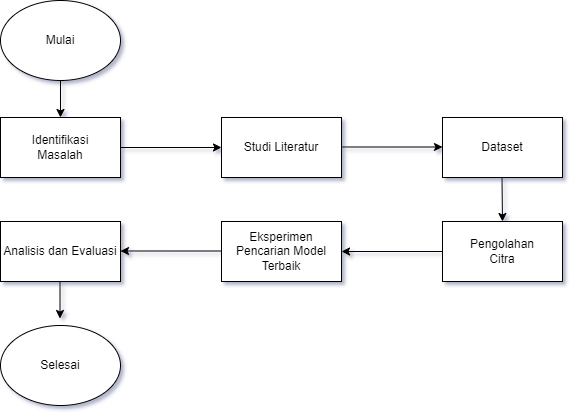
\includegraphics[width=0.8\textwidth]{figures/bab3/Diagram alir penelitian.png}
      \caption{Diagram Alir Penelitian}
      \label{Diagram Alir Penelitian}
      \medskip % spasi vertikal
      \begin{minipage}{0.8\textwidth}
        \centering
        %Sumber: \url{https://idanovinda.medium.com/mengapa-diperlukan-regularisasi-pada-model-neural-network-d622ed98f9a8}
      \end{minipage}
    \end{figure}


    Data yang digunakan merupakan data sekunder dengan format video, oleh sebab itu peneliti tidak melakukan pengambilan data secara langsung. Data akan di ekstrak kedalam bentuk gambar, selanjut beralih ke pemrosesan citra, yang meliputi prapemrosesan dan penambahan data, eksperimen, analisis, dan penilaian. Proses yang akan dilakukan mencakup seluruh rentang dari  pengambilan dataset hingga penilaian dan analisis, semuanya diarahkan dengan tujuan membangun model yang efisien. 
    
    Proses klasifikasi secara umum dimulai dengan eksplorasi data video yang berfokus pada fitur-fitur video yang relevan. Tahap selanjutnya adalah praproses awal, yang meliputi seleksi fitur, penentuan nilai EAR (\textit{Eye Aspect Ratio}) dan MAR \textit{(Mouth Aspect Ratio}), dan konversi data video menjadi data gambar. Sebelum memasuki tahap klasifikasi menggunakan CNN \textit{(Convolutional Neural Network}), data terlebih dahulu menjalani praproses kedua, yaitu proses augmentasi data dan melakukan pembagian data menjadi data latih (\textit{training}) dan set data uji (\textit{testing}).

    Pada tahap klasifikasi, model akan menghasilkan metrik evaluasi seperti akurasi,\textit{ precision}, \textit{recall}, dan \textit{f1-score}. Hasil evaluasi ini kemudian dianalisis dan dievaluasi. Jika hasil evaluasi telah memenuhi kriteria yang ditetapkan, maka proses klasifikasi selesai. Namun, jika hasil evaluasi belum memenuhi kriteria, maka proses klasifikasi akan diulangi dengan kembali ke tahap praproses awal. Setiap tahap dalam proses klasifikasi digambarkan secara visual dalam Gambar \ref{flowchart}.


    \begin{figure}[H]
      \centering
      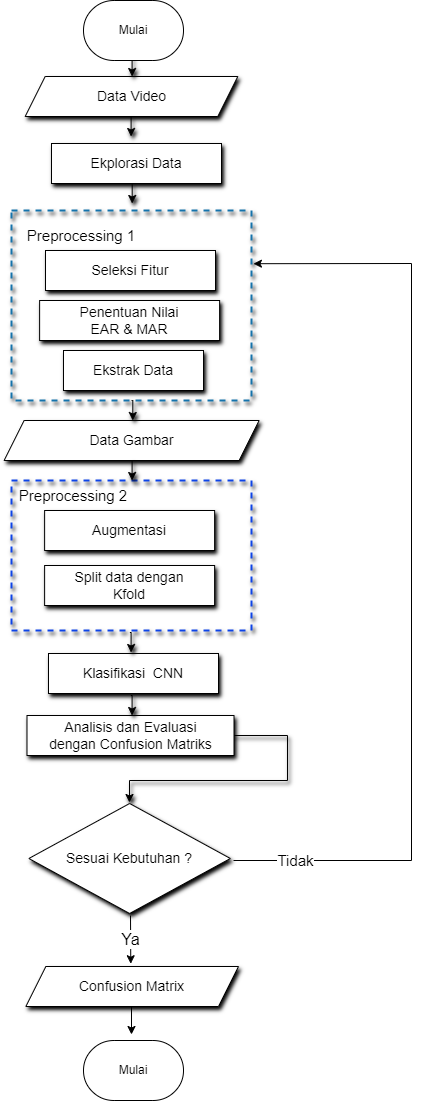
\includegraphics[width=0.6\textwidth]{figures/bab3/1flowchart.png}
      \caption{Gambaran Umum Sistem Klasifikasi}
      \label{flowchart}
      \medskip % spasi vertikal
      \begin{minipage}{0.8\textwidth}
        \centering

      \end{minipage}
    \end{figure}


    

\section{Instrumen Penelitian}

Dalam penelitian ini, proses pelatihan CNN dilakukan dengan menggunakan layanan \textit{Google Colabboration}. Sementara untuk spesifikasi perangkat yang digunakan ditampilkan sebagai berikut.


    \begin{enumerate}
        \item Penelitian ini memanfaatkan perangkat lunak berikut:

        \begin{enumerate}
            \item \textit{Windows 11 x64}
            \item \textit{Python 3.11.4}
            \item \textit{Tensorflow 2.9.1}
            \item \textit{Conda 22.9.0} \item \textit {Dlib 19.22.1}
            \item \textit{Open CV 4.8.1}
            \item \textit{Google Colaboratory}
        \end{enumerate}
        
        \item Penelitian ini memanfaatkan perangkat keras berikut: laptop Lenovo dengan \textit{processor} AMD  A8-7410 \textit{with} AMD Radeon Graphics (4 CPUs),  2.2 GHz, RAM 12 GB DDR3L, dan SSD 256 GB.

    \end{enumerate}
    
\section{Penjabaran Langkah Penelitian}

    Untuk memperjelas setiap langkah-langkah yang telah didefinisikan pada Gambar \ref{Diagram Alir Penelitian}. Berikut ini akan dijabarkan secara rinci tahapan-tahapan yang dilakukan dalam penelitian ini.
    
\subsection{Studi literatur}

    Langkah awal penelitian ini melibatkan pengumplan literatur untuk menghimpun informasi, referensi, konsep dasar, dan pengetahuan yang menjadi dasar penelitian. Proses ini mencakup pencarian dan pembacaan berbagai sumber seperti buku, jurnal, dan artikel yang terkait dengan penelitian ini. Selain itu, dilakukan analisis menyeluruh terhadap penelitian-penelitian sebelumnya untuk memahami berbagai perkembangan penelitian dibidang yang sama.

    
\subsection{Data}

    Data yang dimanfaatkan dalam penelitian ini termasuk dalam kategori data sekunder dengan format video (avi). Sumber data ini berasal dari YAWDD: YAWNING DETECTION DATASET. Dataset ini mencakup pengemudi dengan berbagai karakteristik wajah yang digunakan untuk pengujian algoritma dan model untuk deteksi kantuk, tetapi juga pengenalan dan pelacakan wajah dan 
    mulut. Dalam kumpulan data ini, memberikan anotasi untuk properti-properti berikut (properti ditunjukkan dalam urutan berikut):


    \begin{enumerate}

        \item Video diambil dalam kondisi pencahayaan yang nyata dan bervariasi.
        \item Kamera dipasang di bawah kaca spion depan mobil dan \textit{dashboard} mobil. 
        \item  Setiap peserta memiliki tiga/empat video dan setiap video berisi kondisi mulut yang berbeda seperti normal berbicara/menyanyi, dan menguap. 
        \item Dataset ini menyediakan 316 video yang terdiri dari pengemudi pria dan 
        pengemudi pria dan wanita, dengan dan tanpa kacamata, dari etnis yang berbeda.
        \item Situasi: mengemudi normal (tidak berbicara), berbicara atau bernyanyi saat mengemudi, dan menguap menguap saat mengemudi.



    Contoh dataset yang digunakan ditampilkan pada Gambar \ref{Contoh Dataset} berikut.

    \begin{figure}[H]
        \centering
        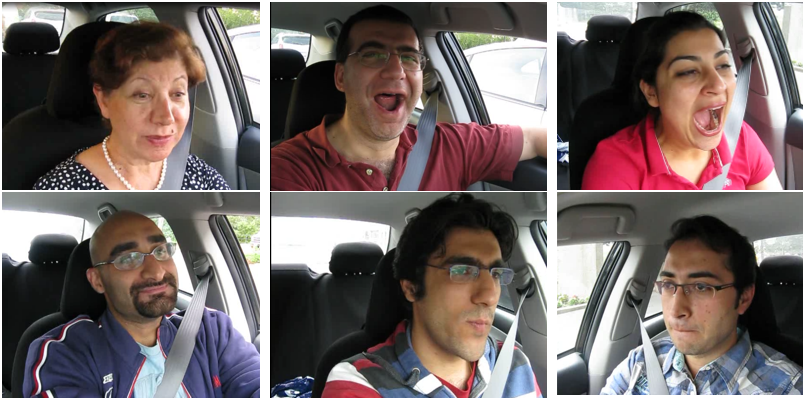
\includegraphics[width=0.85\textwidth]{figures/bab3/image.png}
        \caption{Contoh Dataset}
        \label{Contoh Dataset}
    \end{figure}

        
    
    \end{enumerate}
    
  
    Setelah data dikumpulkan, proses selanjutnya melakukan pengolahan data, di mana video akan diklasifikasi dan diekstrak sesuai dengan kelasnya. Pra-pemrosesan data melibatkan sejumlah tugas, seperti penyesuaian ukuran dan pemotongan bingkai video, normalisasi data, serta ekstraksi fitur-fitur yang relevan dari konten video. Data kemudian dibagi menjadi \textit{subset} untuk keperluan pelatihan, validasi, dan pengujian model. Selain itu, data akan diterapkan pada arsitektur CNN untuk mendeteksi mengantuk pada pengemudi.
    
\subsection{\textit{Preprocessing }Data}
   
    Proses ini terkait dengan ekstraksi data, augmentasi data, pembagian data, ekstraksi fitur citra, dan klasifikasi citra. Tujuannya adalah untuk mencapai efisiensi yang baik dalam pelatihan model, baik dari segi akurasi maupun waktu, sehingga dapat meningkatkan kualitas dan kinerja model, serta memastikan keakuratan hasil.
    
  
\subsubsection{Ekstraksi Data}
    Penelitian ini menggunakan data berformat video (.avi) dengan ukuran 640 $x$ 480 piksel dengan resolusi 30 FPS. Sehingga perlu dilakukan  ekstrak video ke dalam bentuk gambar (.jpg). Eksraksi video ke gambar merupakan langkah penting dalam proses deteksi kantuk. Video diubah menjadi bingkai/gambar, kemudian dilakukan klasifikasi berdasarkan ekstraksi untuk daerah mata dan mulut. Penelitian ini menggunakan \textit{library} Dlib untuk detektor wajah dan 68 \textit{facial landmark predictors} untuk mata dan mulut. Proses ini melibatkan konversi setiap \textit{frame} video menjadi gambar langsung di kelompokkan berdasarkan kelasnya. Nilai EAR (\textit{Eye Aspect Ratio}) dan MAR \textit{(Mouth Aspect Ratio}) akan digunakan dalam klasifikasi pada setiap \textit{frame}.
    
    \begin{enumerate}
        \item     \textit{\textbf{Eye Aspect Ratio (EAR)}} digunakan untuk mengukur keterbukaan mata. EAR dihitung dengan menggunakan rasio jarak antara beberapa\textit{ landmark }mata. Nilai EAR berkisar antara 0 dan 1. Nilai EAR yang mendekati nol menunjukkan bahwa mata tertutup, sedangkan nilai EAR yang mendekati satu menunjukkan bahwa mata terbuka lebar

        \item \textbf{\textit{Mouth Aspect Ratio }}(MAR) digunakan untuk mengukur lebar bukaan mulut. MAR dihitung dengan menggunakan rasio jarak antara beberapa \textit{landmark} di sekitar mulut. Nilai MAR yang mendekati nol menunjukkan bahwa mulut tertutup rapat, sedangkan nilai MAR yang mendekati satu menunjukkan bahwa mulut terbuka lebar. 
    \end{enumerate}

    Untuk lebih jelasnya terkait ekstraksi video ke dalam bentuk foto dengan EAR dan MAR, akan ditampilkan ilustrasi pada Gambar \ref{Alur Ekstraksi Video} berikut.
    
  
    \begin{figure}[H]
        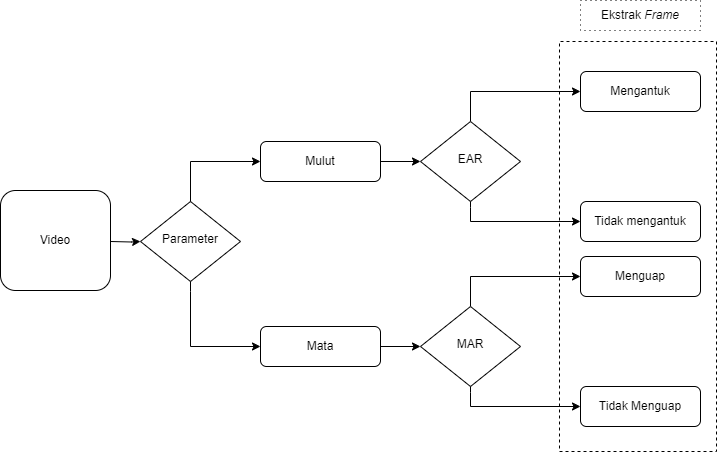
\includegraphics[width=1.0\textwidth]{figures/bab3/procesing.png}
        \caption{Alur Ekstraksi Video}
        \label{Alur Ekstraksi Video}
    \end{figure}

    

    

    
    Setiap data yang diekstrak ke bentuk gambar akan dikelompokkan berdasarkan kelasnya, di mana setiap \textit{frame}nya akan dikelompokkan berdasarkan kelasnya. Kelas pada dataset digunakan berdasarkan kondisi mata dan mulut. Kedua parameter ini akan digunakan untuk mendeteksi kantuk. Mata yang terbuka ditandai dengan nilai EAR yang mengecil dan akan dikelompokkan pada kategori mengantuk untuk setiap \textit{frame}, sedangkan yang lainnya tidak mengantuk. Sementara itu, mulut digunakan untuk mengkategorikan keadaan menguap atau tidak. Nilai MAR yang semakin bertambah menandakan mulut terbuka dan dikategorikan sebagai menguap, sedangkan yang lainnya tidak menguap. Kombinasi dari kedua parameter tersebut akan menghasilkan beberapa kelas yang akan dilatih pada arsitektur CNN. Berikut ini adalah kategori kelas yang akan digunakan. Yang dapat dilihat pada Tabel \ref{Keterangan Anotasi Kelas} berikut.


    
    \begin{table}[h]
        \centering
        \caption{Keterangan Anotasi Kelas}
        \begin{tabular}{cccc}
            \hline
            \textbf{Kondisi Mata} & \textbf{Kondisi Mulut} & \textbf{Hasil} \\
            \midrule Mengantuk & Menguap &  Mengantuk dan Menguap\\
                     Mengantuk & Tidak Menguap &  Mengantuk tidak Menguap \\
                     Tidak Mengantuk & Menguap &  Menguap tidak Mengantuk\\
                
        
            \bottomrule
        \end{tabular}
        \label{Keterangan Anotasi Kelas}
    \end{table}
    

\subsubsection{Augmentasi Data}

    Setelah video di ekstraksi ke bentuk gambar, perlu dilakukan proses pengolahan citra dari data yang sebelumnya diperoleh. Proses augmentasi adalah teknik yang sering digunakan untuk meningkatkan ukuran kumpulan data tanpa memerlukan pengambilan data tambahan. Teknik ini melibatkan pengambilan data selama tahap pengumpulan dan persiapan data sebelumnya. Salah satu pendekatannya melibatkan penerapan transformasi pada data gambar asli. Transformasi ini dapat dilakukan berupa rotasi, pemberian \textit{noise}, penskalaan, pemotongan, dan penambahan nilai piksel melalui modifikasi kecerahan. Semuanya ini dilakukan untuk meningkatkan ukuran dan variasi data. Teknik ini dilakukan dengan tujuan untuk mengurangi resiko \textit{overfitting}.

\subsubsection{\textit{Splitting} Data}
   Data akan dipisahkan menjadi tiga kategori: data \textit{test}, data \textit{validation}, dan \textit{train}. Data \textit{train} ditujukan untuk memfasilitasi proses pembelajaran model selama fase pelatihan. Data \textit{validation} digunakan untuk memberikan informasi yang tidak bias kepada model. Selanjutnya, data ini secara konsisten digunakan selama percobaan, sehingga model sering terpapar dengan data tersebut. Hasil dari eksperimen yang dilakukan secara tidak langsung mempengaruhi model melalui data \textit{validation}. 
   Data pengujian digunakan untuk menilai kinerja model dengan data baru yang belum pernah dilihat, yang digunakan hanya sekali pada eksperimen. Pembagian ini diimplementasikan dengan tujuan untuk mencapai distribusi yang seimbang dan untuk mengoptimalkan kemampuan generalisasi model.

\subsection{Desain Arsitektur CNN}

    Merancang struktur yang efektif dengan mengekstrak fitur penting dari data gambar disebut sebagai desain arsitektur \textit{Convolutional Neural Network} (CNN). CNN adalah tipe arsitektur yang umum digunakan dalam pemrosesan gambar dan berbagai aplikasi pengenalan pola. Tujuan dari klasifikasi ini adalah untuk menghasilkan luaran yang menunjukkan keadaan pengendara sesuai dengan kelas yang telah di tetapkan. Seperti mengantuk dan menguap, mengantuk dan tidak menguap, menguap tidak mengantuk.  Proses diilustrasikan pada Gambar \ref{Proses Convolusional Neural Network} berikut.
 
     \begin{figure}[H]
      \centering
      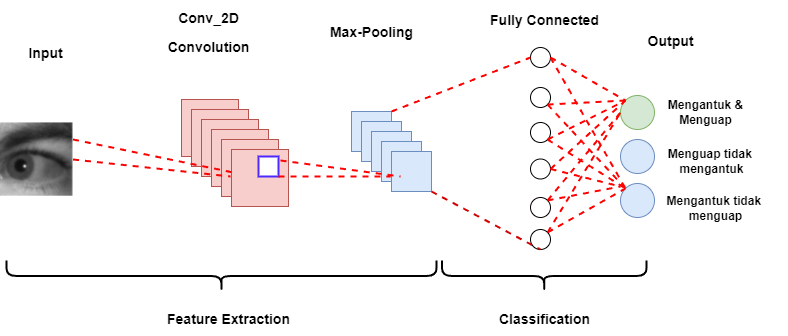
\includegraphics[width=0.85\textwidth]{figures/bab3/cnn_arsitektur.png}
      \caption{Proses \textit{Convolusional Neural Network}}
      \label{Proses Convolusional Neural Network}
    
      \medskip % spasi vertikal
      \begin{minipage}{0.8\textwidth}
        \centering

      \end{minipage}
    \end{figure}

    Proses pelatihan menggunakan data berlabel yang telah dipisahkan ke dalam kumpulan data \textit{train}, \textit{test}, dan \textit{validation}. Kemudian akan dilakukan \textit{tuning hyperparameter} seperti \textit{activation layer}, \textit{learning rate} dan \textit{optimizer}. Augmentasi data dilakukan untuk memodifikasi data gambar sedemikian rupa sehingga, meskipun komputer menganggap gambar telah diubah sebagai gambar baru, manusia masih dapat mengenalinya sebagai gambar yang sama. Selanjutnya, hasil pemrosesan di evaluasi dan diuji pada tahap perbandingan model untuk menentukan model yang optimal untuk mengklasifikasikan dataset.

\subsection{\textit{Traning} Data}

    Setelah arsitektur CNN disesuaikan, penulis akan melatih model menggunakan data yang telah melalui tahap \textit{preprocessing}. Proses pelatihan melibatkan penyesuaian bobot dan \textit{bias} pada setiap lapisan CNN agar mampu mengenali citra dengan akurasi yang tinggi. Pada saat pelatihan di terapkan teknik \textit{early stopping} hal ini bertujuan untuk mencegah \textit{overfitting} dan mengoptimalkan waktu pelatihan. Teknik ini bekerja dengan menghentikan proses pelatihan lebih awal jika performa model pada data validasi tidak meningkat setelah sejumlah epoch tertentu.
    
    Untuk membuat model yang dapat mendeteksi kantuk serta dapat melakukan prediksi dengan efektif, dilakukan beberapa eksperimen yang saling berkaitan dan berhubungan satu sama lain.

     \begin{enumerate}
  
        \item Eksperimen Ke-1

        Eksperimen pertama dilakukan untuk menguji berbagai nilai atau jenis \textit{hyperparameter}. \textit{Hyperparameter} yang diuji adalah nilai atau jenis dari \textit{hyperparameter} yang digunakan dalam model. Model yang dihasilkan dari setiap kombinasi nilai atau jenis \textit{hyperparameter} kemudian dievaluasi untuk mengukur akurasi. \textit{Hyperparameter} yang menghasilkan model dengan akurasi paling optimal kemudian digunakan pada eksperimen selanjutnya. Rentang nilai atau jenis \textit{hyperparameter} yang diuji dapat dilihat pada Tabel \ref{Pengujian Parameter} berikut.



            \begin{table}[h]
            \centering
            \caption{Pengujian Parameter}
            \begin{tabular}{cccc}
                \toprule
                \textbf{} & \textbf{Parameter} \\
                \midrule
                      
                          \textit{Activation}  &  \textit{ReLU, Softmax, Sigmoid }\\
                         \textit{Optimizer} &  \textit{Adam, SGD} \\
                          \textit{Learning Rate} &  0.01, 0.001, 0.0001 \\
            
                \bottomrule
            \end{tabular}
            \label{Pengujian Parameter}
        \end{table}
        
        
        \item Eksperimen ke-2

        Eksperimen kedua merupakan eksperimen yang dilakukan untuk menguji performa model dengan menggunakan arsitektur CNN dan \textit{hyperparameter} yang telah dioptimalkan. Model yang digunakan pada eksperimen ini adalah model yang dihasilkan dari eksperimen sebelumnya. Data uji digunakan untuk mengevaluasi performa model dalam memprediksi data yang belum pernah dilihat sebelumnya.

        
       
    \end{enumerate}




 

\section{Evaluasi Hasil}

    Dalam penelitian ini, kinerja pengenalan atau klasifikasi diukur dengan menggunakan teknik yang telah banyak diterapkan dalam skenario penelitian serupa. Selain itu, pendekatan \textit{confusion matrix} juga diterapkan, seperti yang terlihat pada Gambar \ref{Confusion Matrix}, karena data yang digunakan adalah data berlabel. Pada tahap ini, Peneliti mengukur performa model CNN menggunakan \textit{confusion matrix} yang mencakup \textit{accuracy}, \textit{recall},\textit{ precision}, dan \textit{f-1 score}.

    \textit{True Positive} (TP) menunjukkan jumlah gambar pengemudi yang mengantuk yang diidentifikasi dengan benar oleh model. Hal ini terjadi ketika model secara akurat menilai gambar pengemudi yang disediakan. Sebaliknya, \textit{False Positive} (FP) adalah jumlah data yang salah yang diklasifikasikan sebagai benar. \textit{False Negative} (FN) menunjukkan jumlah data yang benar yang salah diklasifikasikan sebagai salah. Hal ini terjadi ketika model gagal untuk secara akurat menilai gambar yang diberikan tentang pengemudi yang mengantuk, sehingga menghasilkan output yang tidak sesuai dengan input yang diberikan. Terakhir, \textit{True Negative} (TN) menunjukkan jumlah data yang sebenarnya salah yang berhasil diklasifikasikan oleh model.
    
    Keempat kriteria penilaian dalam \textit{confusion matrix }penelitian ini didasarkan pada kemampuan model dalam menilai setiap gambar berkendara yang telah diberi label sebelumnya. Semua prosedur eksperimental yang berhasil merupakan titik fokus utama dalam penyelidikan ini. Hasil dari setiap percobaan dibandingkan secara komprehensif untuk menyimpulkan analisis. Setiap eksperimen diteliti dan dinilai dengan cermat untuk menentukan potensinya dalam mencapai performa model tertinggi.


